\header{
    \headtitle{Le con et la bouteille} \label{le-con-et-la-bouteille}
    %
    
    \insertComment{Parue en 1866 dans "Le panier aux ordures".}{}
}

\enluminure{4}{\href{https://www.youtube.com/watch?v=L-pjJoDMmkc}{L}}{argue} des pédants et des sots
\\Qui viennent chagriner notre âme,
\\Que fit Dieu pour guérir nos maux
\\Les vieux vins et les jeunes femmes !
\\Il créa pour notre bonheur
\\Le sexe et le jus de la treille :
\\Aussi, je viens en son honneur
\\Chanter les cons et les bouteilles. \bissimple
\\\\Dans l'Olympe, séjour des Dieux,
\\On boit, on patine les fesses,
\\Et le nectar délicieux
\\N'est que le foutre des déesses !
\\Si j'y vais, jamais Apollon
\\Ne charmera plus mon oreille,
\\De Vénus, je saisis le con,
\\De Bacchus, je prends la bouteille. \bissimple
\\\\Dans les bassinés féminins,
\\Quand on a brûlé des amorces,
\\Quelques bouteilles de vieux vin
\\Au vit rendent toute sa force,
\\Amis, plus on boit, plus on fout :
\\Un buveur décharge à merveille.
\\Aussi le vin pour dire tout,
\\C'est du foutre mis en bouteille! \bissimple
\\\\On ne peut pas toujours bander,
\\Du vit, le temps borne l'usage,
\\On se fatigue à décharger,
\\Mais, amis, on boit à tout âge!
\\Quant aux vieillards, aux froids couillons,
\\Qu'ils utilisent mieux leurs veilles,
%ici Veille signifie veillée (la soirée)
% les vieux profitent du soir en buvant en non en baisant
\\Quand on n'peut plus boucher de cons,
\\On débouche au moins des bouteilles! \bissimple
\breakpage
Mais, hélas, depuis bien longtemps,
\\Pour punir nos fautes maudites,
\\Le Bon Dieu fit des cons trop grands
\\Et des bouteilles trop petites !
\\Grand Dieu, fais, nous t'en supplions,
\\Par quelque nouvelle merveille,
\\Toujours trouver le fond du con,
\\Jamais celui de la bouteille ! \bissimple
\bigskip
\begin{center}
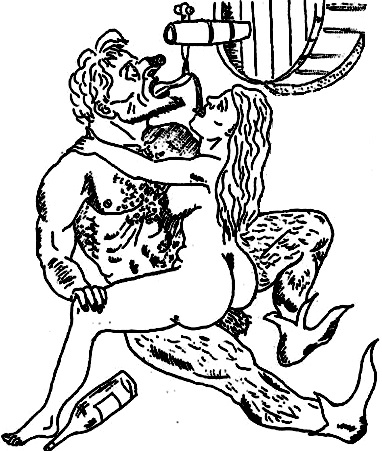
\includegraphics[width=0.9\textwidth]{images/le_con_et_la_bouteille.jpg}
\end{center}

\breakpage